\section{Experimental Setup}
\label{sec:experimentalSetup}

To create a fair comparison of the various wake up approaches, it is necessary to ensure a high control of consistency and repeatability of the input sensor data. Unfortunately, this is very difficult to achieve during live experiments performed by human subjects. Instead, we opted to collect accelerometer traces and run trace-based simulations.

Additionally, our simulations requires the availability of ground truth in order to accurately compute metrics such as event of interest detection precision and recall. Annotating accelerometer traces collected from human subjects with ground truth information about the performed actions is both extremely time-consuming and prone to errors. Instead, we chose to use a robot to perform a set of actions and simultaneously keep a log of ground truth information about the performed actions.

The use of a robot could have enabled us to run live experiments because performing the same sequence of actions multiple times would result in similar accelerometer traces. We opted not to do so for several reasons. Each run takes upwards of an hour to execute. Our goal was to obtain results for a multitude of wake-up approaches, each under multiple parameter configurations. Additionally, we wanted to reduce the impact of outliers on our results by running each experiment on a multitude of robot action sequences. The combination of all action sequences and wake-up configurations would have required over a year of continuous live experimentation. Running trace-based simulations allows us to perform an exhaustive exploration of the parameter configuration space. Moreover, taking fine grain power consumption measurements while the robot is in motion is not trivial. Nonetheless, this is part of our future work.

The use of a robot significantly limits the set of actions that can be performed in our experiments. Since we are mainly interested in actions that would normally be performed by humans, we tried to configure the robot to perform actions with similar acceleration signatures. We decided upon a set of 4 actions: walking, headbutts and two stance transitions. Robot walking has a similar acceleration signature as its human counterpart, though at a much lower intensity. The headbutts are meant to represent very infrequent human actions such as falling. We found that robot stance transitions between the normal and sitting postures are very similar in their acceleration signature as humans sitting down and standing up.

\begin{figure}[t]
	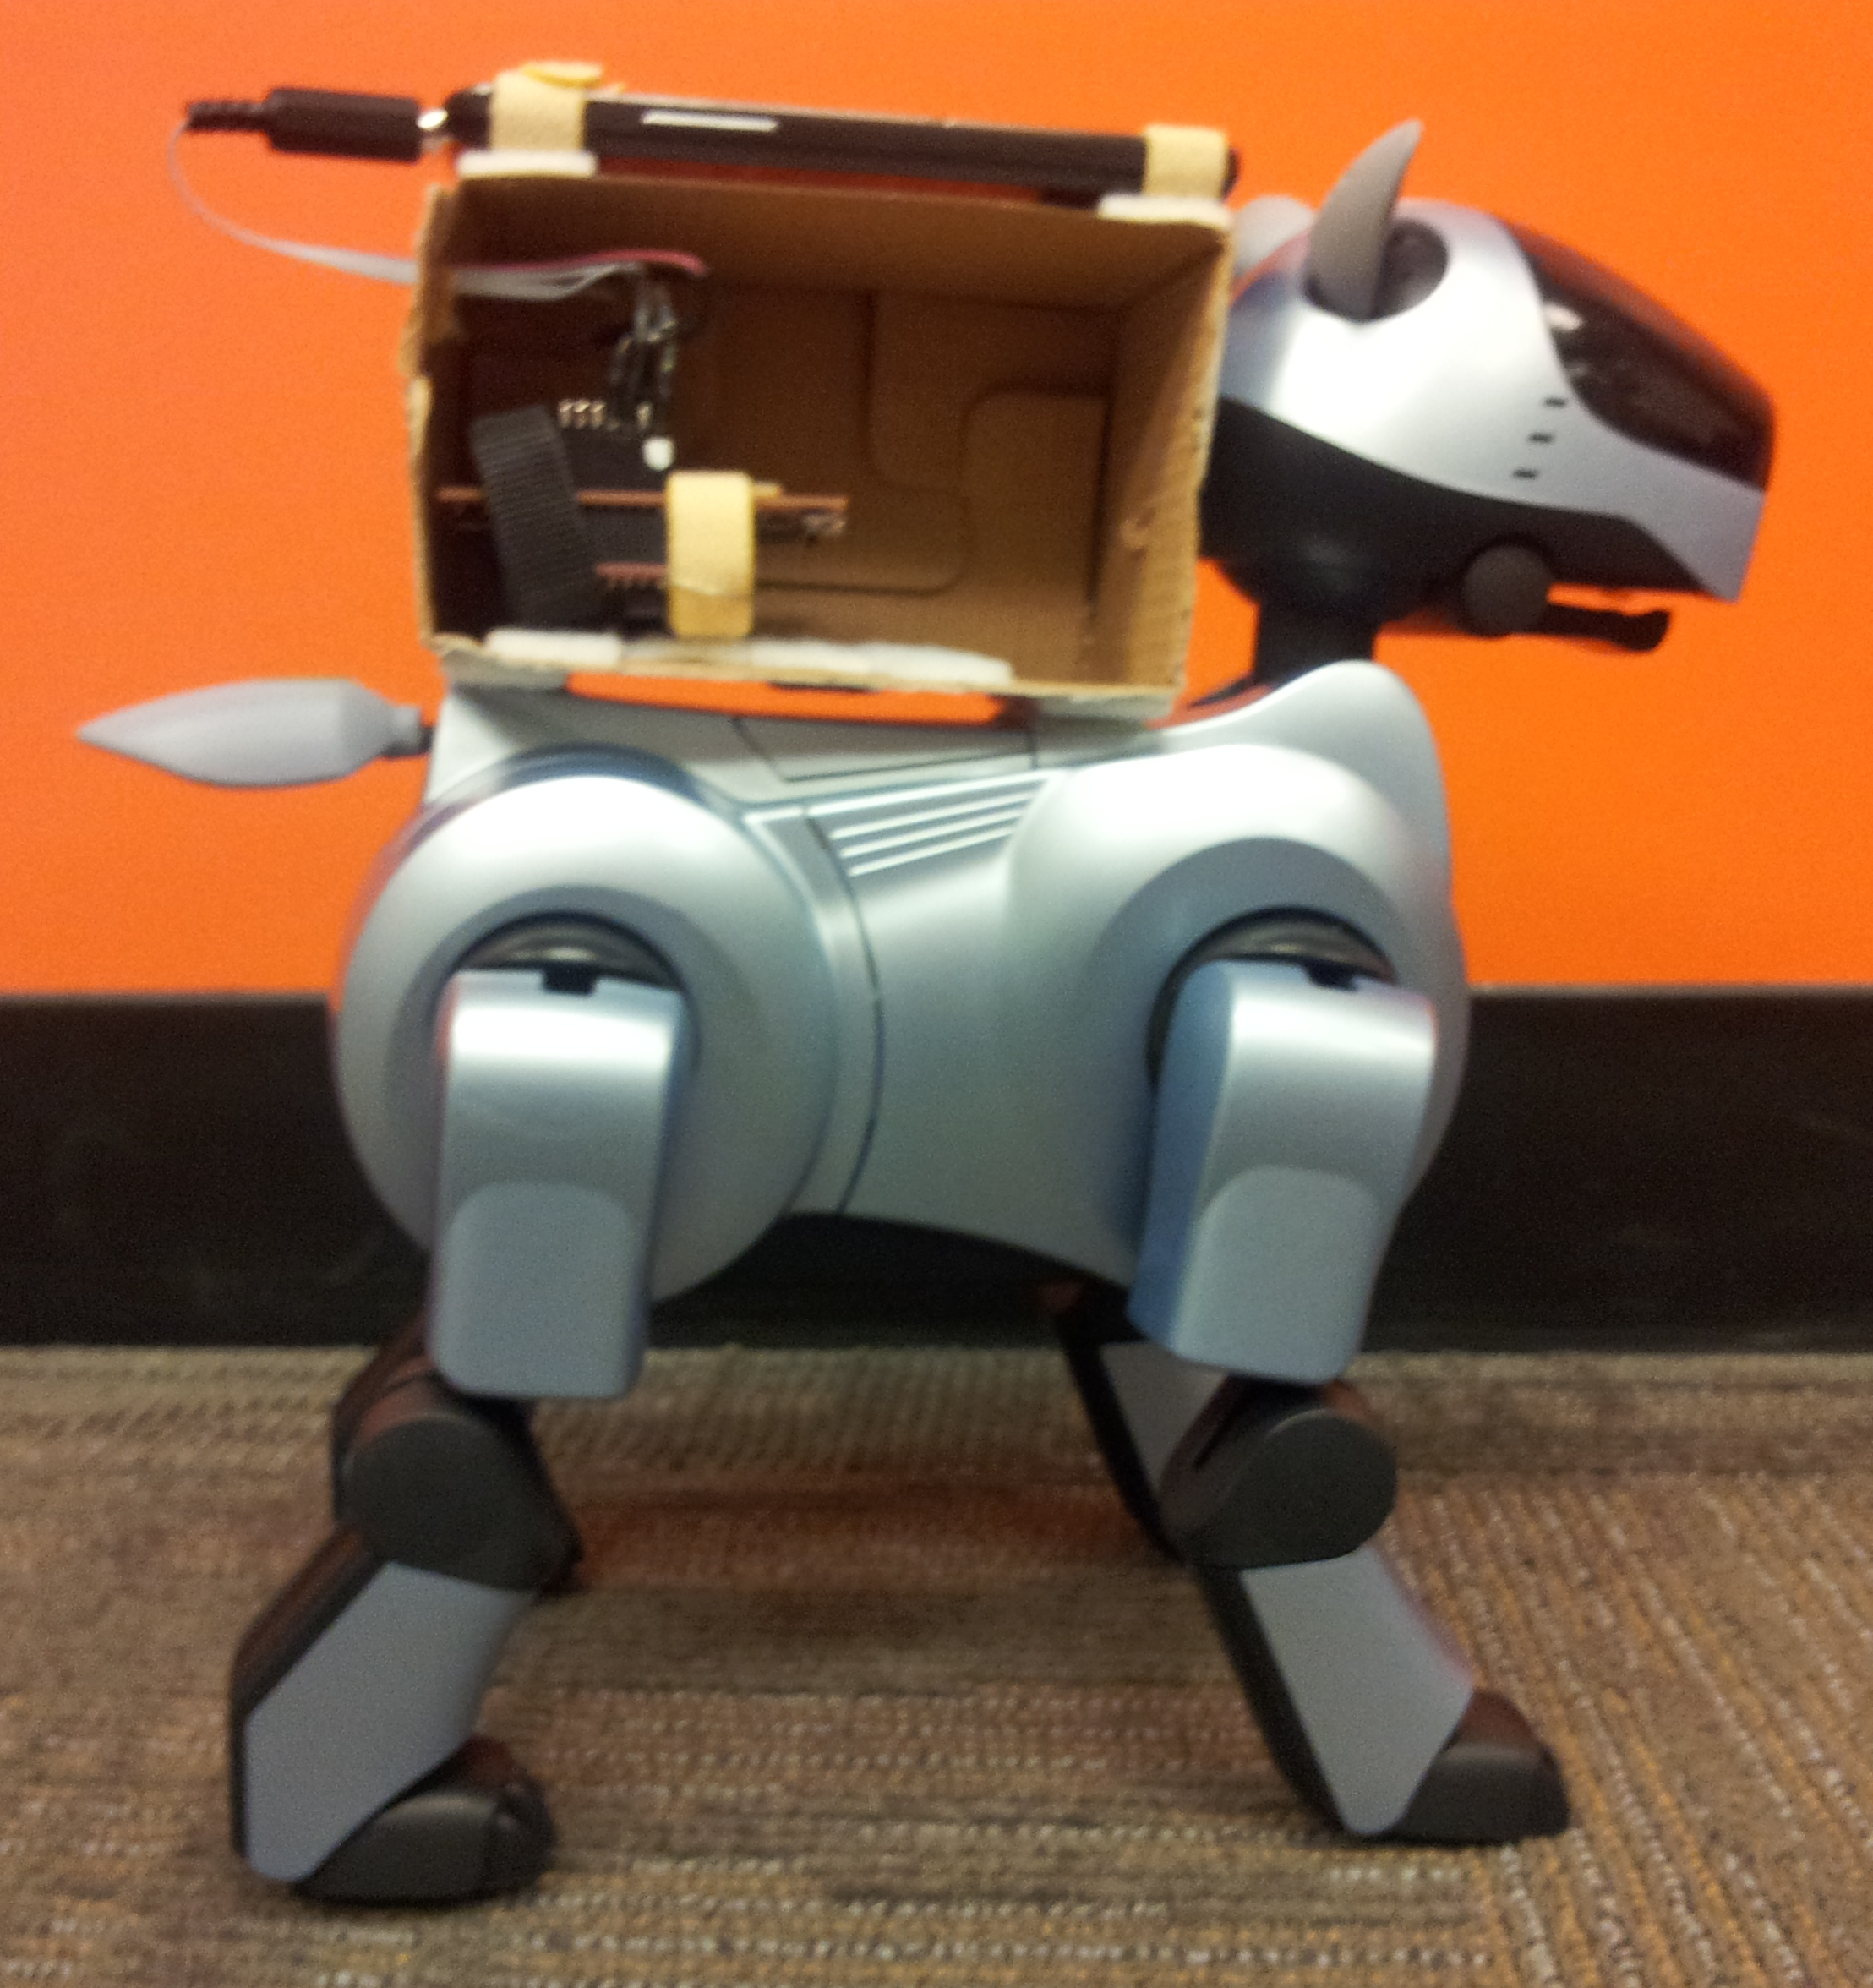
\includegraphics[width=8.5cm]{aibo_ers_210.jpg}
	\caption{AIBO ERS 210 robot used to collect the accelerometer traces}
	\label{fig:aibo}
\end{figure}

To collect the accelerometer traces for our experiments we used an AIBO ERA 210 robot (Figure \ref{fig:aibo}). The robot would perform a sequence of actions and record timestamps for the beginning and end of each action. The set of performed actions and timestamps were outputted to a log file that can be used by the simulator as ground truth. To record the accelerometer trace, we attached a Google Nexus 4 to the back of the dog and ran an application that collected all the accelerometer readings for the duration of the circuit.

\begin{figure}[t]
	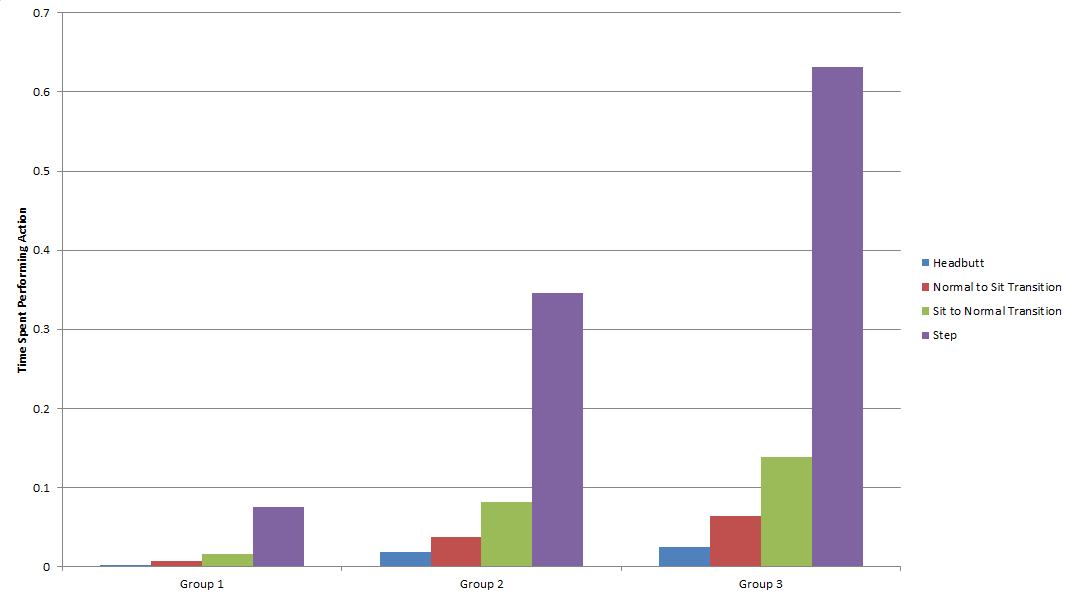
\includegraphics[width=8.5cm]{action_times.png}
	\caption{Time spent performing actions of specific types as a percentage or trace length}
	\label{fig:actionTimes}
\end{figure}

The level of activity can vary significantly between mobile device users. For example, the mobile device of an individual working in an office environment may experience low levels of motion (e.g. sitting on a desk for extended periods of time), while the mobile device of someone constantly in motion (e.g. bike courier) may only experience short period at rest. In our experiments we wanted to cover a wide range of activity level. We divided our traces into 3 groups based on activity level. Groups 1, 2 and 3 contain traces in which the robot performs actions approximately 10\%, 50\% and 90\% of the time, respectively. Within each trace, we also wanted the amount of time each action type is being performed to vary considerably. Figure \ref{fig:actionTimes} shows the average amount of time each action is being perform for the traces in each group, as a percentage of the average trace length.

We implemented 3 applications that attempt to detect the 4 different actions from the accelerometer readings in each trace. A first application looks for local maxima within a certain range in the x-axis acceleration to detect steps taken by the robot. Similarly, the second application looks for local minima within a range in the y-axis acceleration to detect headbutt actions. The third application monitors changes in the acceleration due to gravity on the y and z axes in order to detect stance transitions between a normal posture and sitting. All 3 applications pass the accelerometer data they are interested in through low-pass filters based on Fast-Fourier Transformations.

\subsection{Metrics}
In our evaluation we are investigating several metrics:

\begin{enumerate}
\setlength{\itemsep}{-3pt}  

\item the power consumption of the system

\item the recall of the event of interest

\item the precision of event of interest detection

\item the time delay incurred before the application becomes aware that an event of interest has occurred

\item the precision of device wake-ups

\end{enumerate}

Recall is the fraction of events of interest that have been successfully detected. We calculate event of interest recall by dividing the number of true positives by the total number of performed events of interest as indicated by the ground truth data. Precision is the fraction of the detected events of interest that are present in the ground truth. For a particular event of interest we calculate precision by dividing the number of true positives by the number of detected events of interest of that type. Device wake-up precision is a measure of how often the device unnecessarily wakes up (i.e. wakes up and does not detect an event of interest).

\subsection{Trace-based Simulator}

Each collected accelerometer trace is an ordered set of accelerometer readings. Each reading contains the x-, y- and z-components of the acceleration vector and a timestamp indicating  when the reading was produced.

For each run, the simulator takes the following inputs:

\begin{enumerate}
\setlength{\itemsep}{-3pt}  

\item a parametarized wake-up approach

\item a file containing the accelerometer readings, sorted by timestamp

\item a file containing information about ground truth

\end{enumerate}

The simulator processes the readings one at a time, similarly to how a mobile device would receive accelerometer readings in real-time, as they are produced by the sensor. Based on the wake-up approach, the simulator determines which of the readings would cause the device to wake-up. Also, the simulator determines what readings need to be sent to the running application(s). At the end of the run, the simulator outputs relevant metrics such as:

\begin{enumerate}
\setlength{\itemsep}{-3pt}  

\item amount of time the device would have been awake

\item total number of device wake-up

\item number of wake-ups that did not result in an event of interest being detected

\item true positives, false positives and false negatives for each event of interest

\item recall and precision for each event of interest

\end{enumerate}

\subsection{Power Consumption Model}

To complement our simulator, we created a model to estimate the power consumption for each of our simulator runs. The model is based on real power measurements presented in section \ref{sec:prototype}. The inputs of the model are the amount of time the device is awake, the amount of time it is asleep and the number of transitions between the two states. Based on these values, the energy model outputs the average power consumption over the duration of the trace.

\subsection{Baseline}

\begin{figure}[t]
	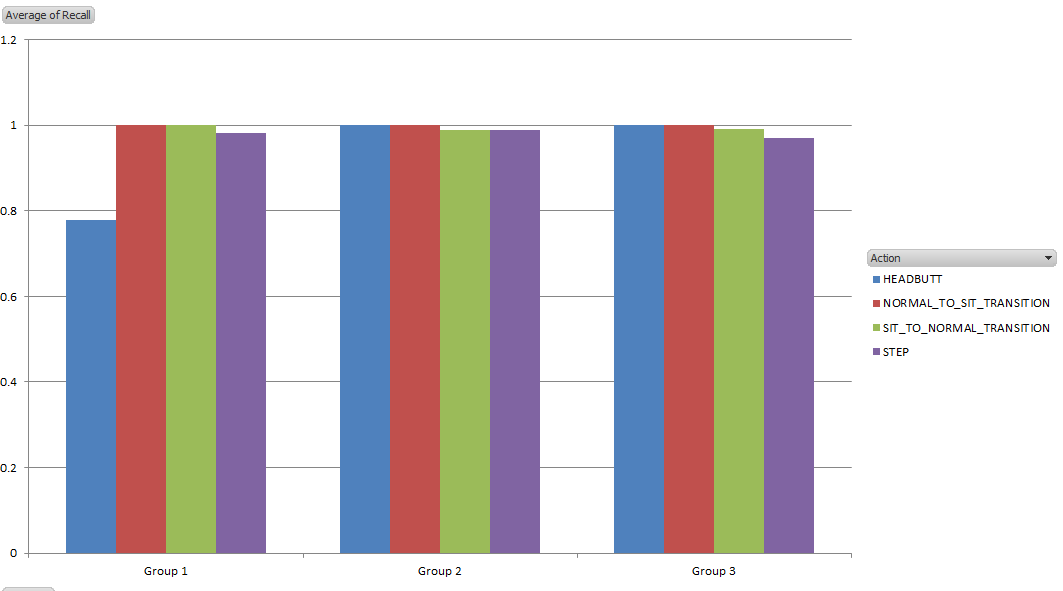
\includegraphics[width=8.5cm]{aa_recall_by_group.png}
	\caption{Always Awake: Recall by Group}
    	\label{fig:aaRecallByGroup}
\end{figure}


\begin{figure}[t]
	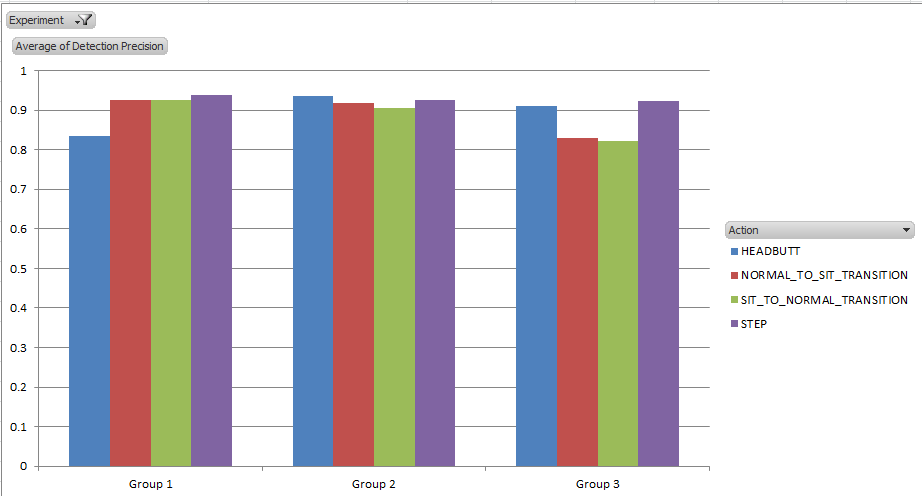
\includegraphics[width=8.5cm]{aa_precision_by_group2.png}
	\caption{Always Awake: Detection Precision by Group}
    	\label{fig:aaPrecisionByGroup}
\end{figure}

In the Always Awake approach, the device is presumed to be awake for the entire duration of the trace and all of the collected accelerometer readings are passed to the applications. We are using the Always Awake approach as a baseline to compare all the following wake-up approaches. Additionally, the Always Awake simulations show the accuracy of the implemented applications in terms of event of interest detection precision and recall. Figure \ref{fig:aaRecallByGroup} shows the recall of each of the events of interest averaged over the traces in each group. We note that with the exception of the headbutt action in Group 1, the event of interest recall is above 95\% for all actions and groups. The headbutt action in group 1 appears to be an outlier because Group 1 contains traces with the least amount of actions and headbutts are the scarcest actions, occurring only about once per trace. Figure \ref{fig:aaPrecisionByGroup2} shows the detection precision of each of the events of interest averaged over the traces in each group. For all cases, the applications achieved a detection precision above 82\%.

The power consumption using this approach is equivalent to the power consumed by the device in the awake state. In the case of the Nexus 4 used in our experiments, the power consumption is 323 mW.

